\section{Rezultati}

V tem poglavju si bomo ogledali nekaj rezultatov uspešnosti različnih modelov. Za vsako kombinacijo števila ovčarjev, ovc, modela gibanja ovc in modela vodenja ovčarja smo naredili 100 simulacij. Na sliki~\ref{fig:prezivetvena} si lahko ogledamo povprečen delež ovc na pašniku ob določenem času do konca simulacije pri 180 sekundah pri vodenju psa z ročno razvitim modelom. Hitro opazimo, da so si rezultati pri Str{\"o}mbomovem in popravljenem Str{\"o}mbomovem modelu gibanja ovc zelo podobni. Ovčar je najuspešnejši pri Ginellijevem modelu. Več ovčarjev običajno pomeni večjo uspešnost. Pri tem je vpliv začetne razdalje najbližjega ovčarja do črede predvsem pri večjih čredah praktično zanemarljiv.

\begin{figure}[ht]  % ali t za na vrhu ali h! za točno tukaj
	\centering
	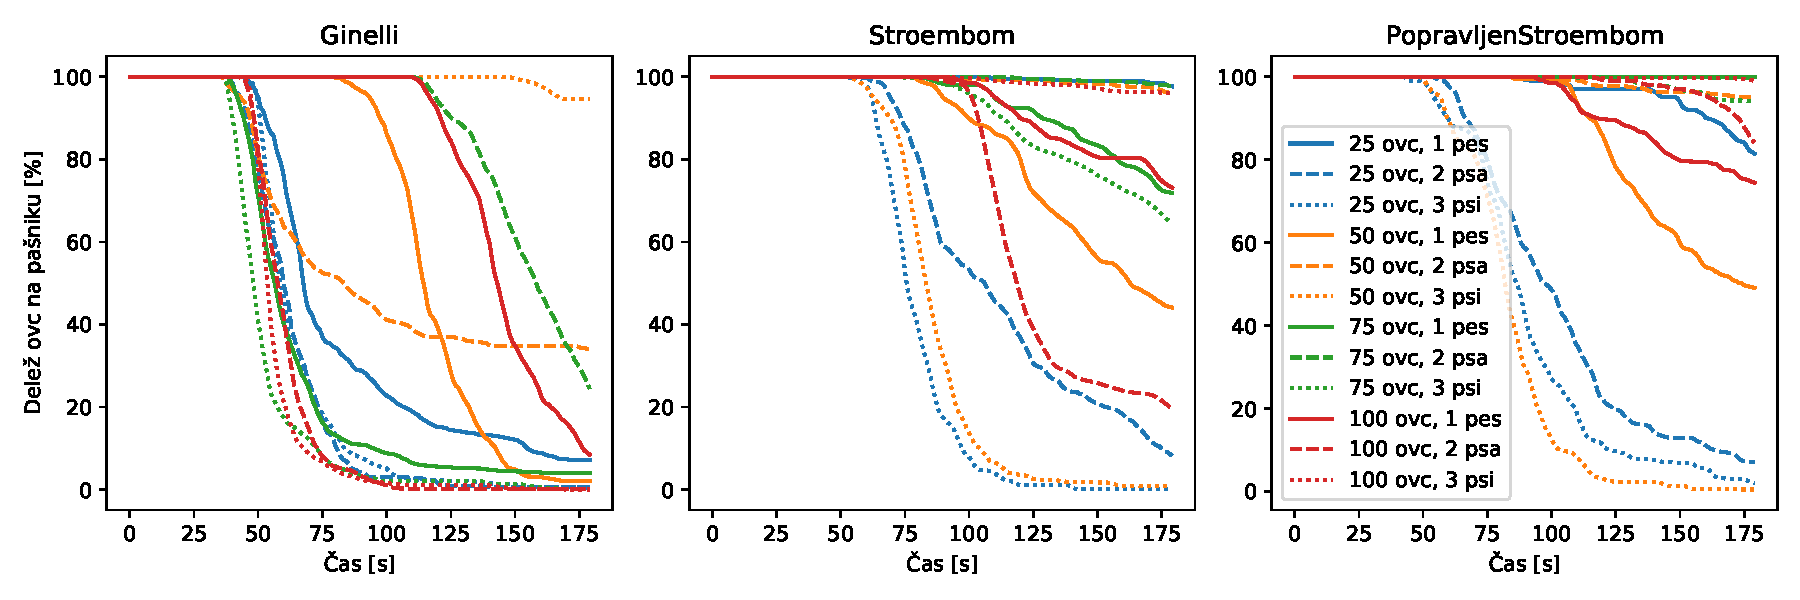
\includegraphics[width=\textwidth]{../poglavja/grafi/prezivetvena-Voronoi.pdf}
	\caption[Delež ovc na pašniku skozi čas]{Delež ovc na pašniku skozi čas za ročno razvit model vodenja ovc. Legenda je za vse grafe enaka in se nahaja le na desnem grafu.} % narejena je s programom Inkscape
	\label{fig:prezivetvena}
\end{figure}

\subsection{Iskanje optimalnega gena}

Na slikah~\ref{fig:fit}-\ref{fig:Ge-gen2} si bomo ogledali nekaj opazovanih lastnosti, kako so se spreminjale skozi generacije. Na vseh grafih temno modra krivulja predstavlja mediano vrednosti izbrane lastnosti, rdeči črti predstavljata ekstremne vrednosti, vmes pa je poleg mediane tudi temnejši moder pas, ki se razprostira od 15. do 85 percentila. Zelena črta predstavlja mediano vrednosti za ročno razviti model, oranžna črta pa predstavlja začetek državnega tekmovanja. V tem delu se bomo pri izrisovanju osredotočili le na Ginellijev in Str{\"o}mbomov model ovc.

Na sliki~\ref{fig:fit} vidimo gibanje ocenjene uspešnosti gena izračunane po formuli~\eqref{eq:genetski}, na sliki~\ref{fig:maxt} trajanje posamezne simulacije skozi generacije, na sliki~\ref{fig:uspeh} delež ovc v staji ob koncu simulacije in na sliki~\ref{fig:Ge-gen2} si lahko ogledamo gibanje genotip drugega parametra $r_a$ , ki predstavlja faktor za dovoljeno velikost črede.

Na nobeni izmed slik ni opaziti pozitivnega pomena državnega tekmovanja, saj so na državnem tekmovanju večinoma le še geni, ki imajo dovolj visoko povprečno in minimalno uspešnost. Poleg tega je v tej točki variabilnost genoma že zelo majhna.

\begin{figure}[H]  % ali t za na vrhu ali h! za točno tukaj
	\centering
	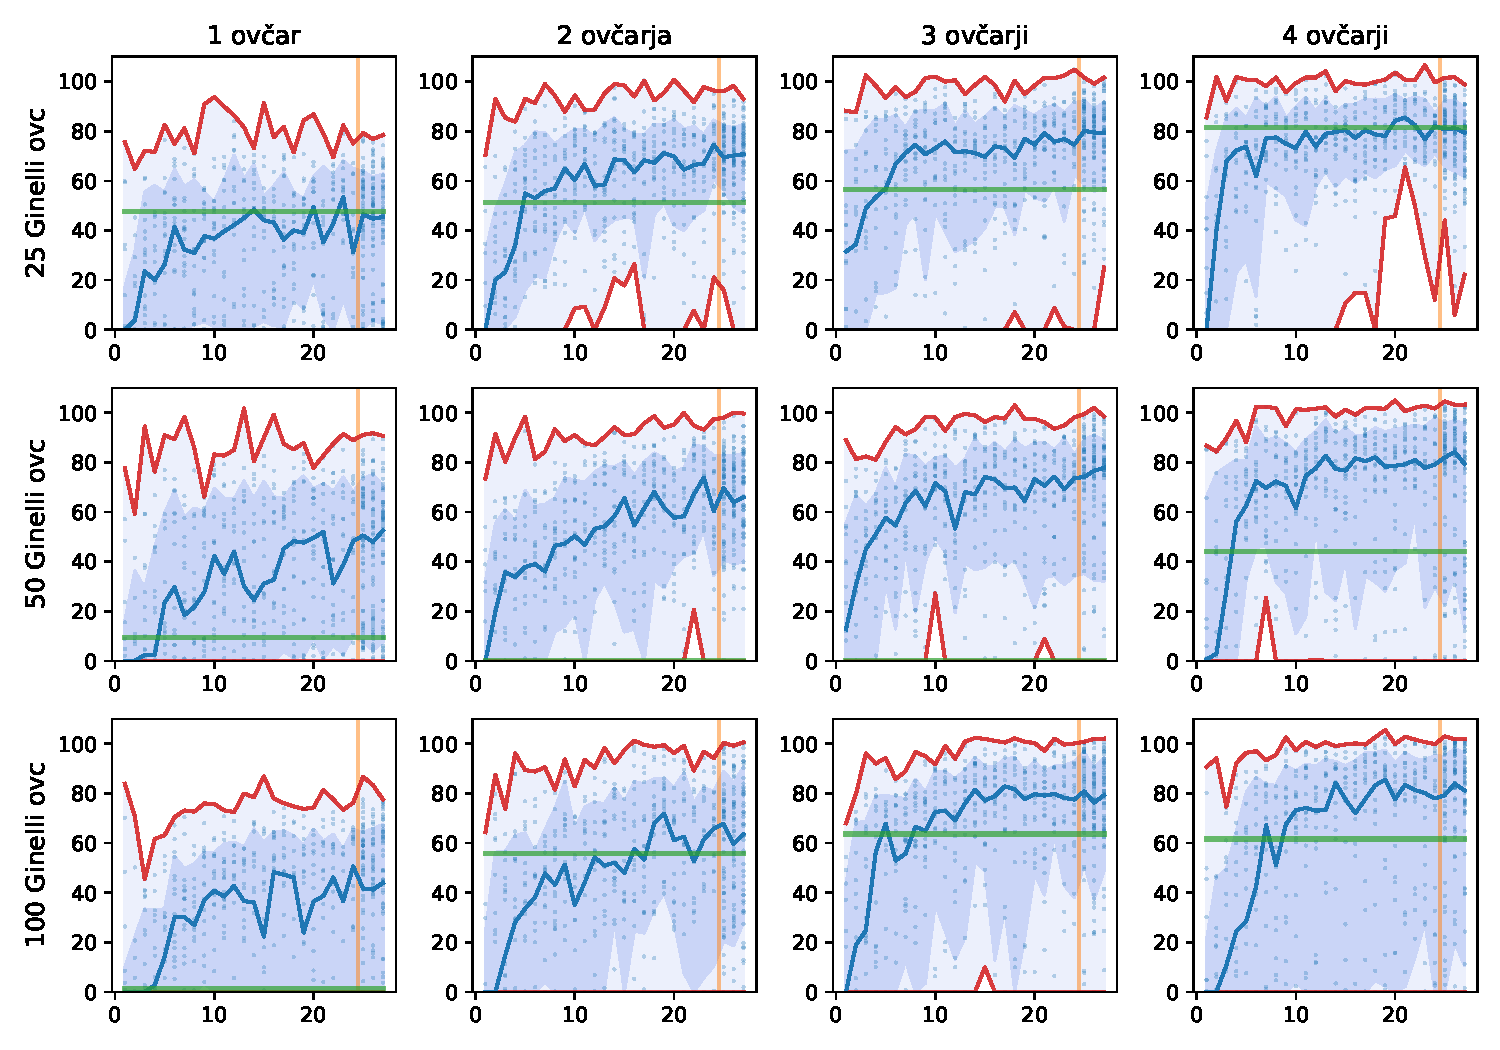
\includegraphics[height=0.4\textheight]{../poglavja/grafi/Ginelli-evolucija-Fitness.pdf}
	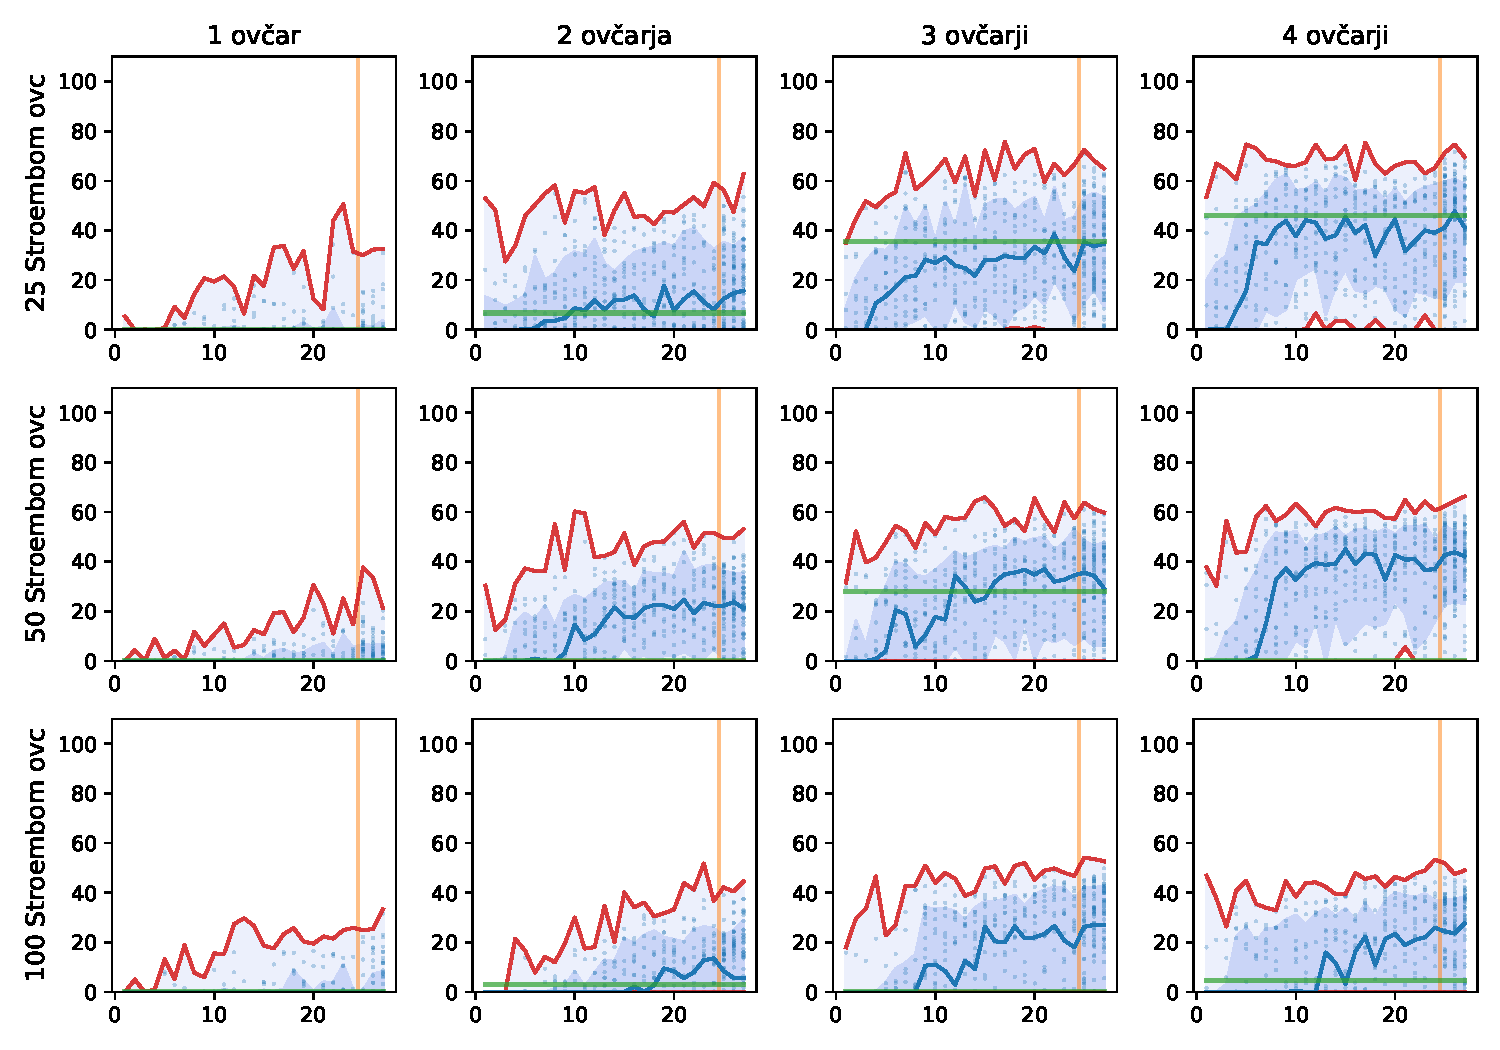
\includegraphics[height=0.4\textheight]{../poglavja/grafi/Stroembom-evolucija-Fitness.pdf}
	\caption[Uspešnost skozi generacije]{Uspešnost skozi generacije. Opazimo, da se praviloma hitro poveča. Pri tem je na koncu uspešnost običajno vsaj primerljiva z ročno razvitim modelom. Zelene črte pogosto ne vidimo, ker je več kot polovica simulacij v nekaterih primerih neuspešnih. Vodenje ovc po Ginellijevem modelu se zdi veliko lažje za naš model vodenja, saj se hitro nauči dobrega gena za poljubno velikost črede ali število ovčarjev.} % narejena je s programom Inkscape
	\label{fig:fit}
\end{figure}

\begin{figure}[H]  % ali t za na vrhu ali h! za točno tukaj
\centering
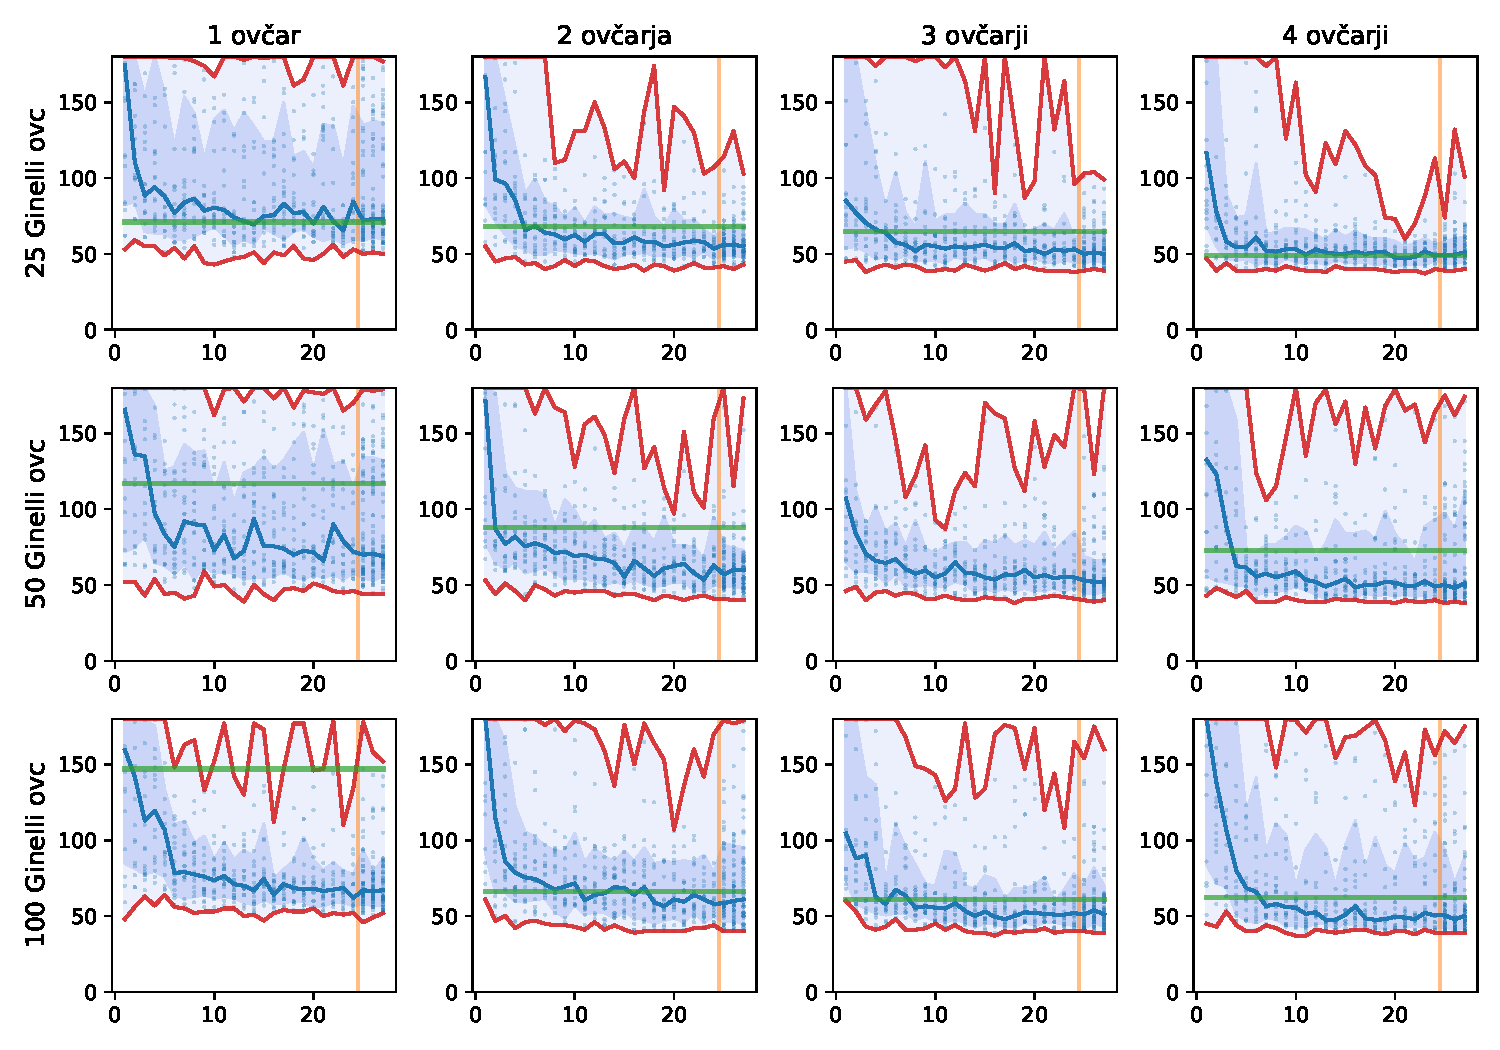
\includegraphics[height=0.4\textheight]{../poglavja/grafi/Ginelli-evolucija-MaxT.pdf}
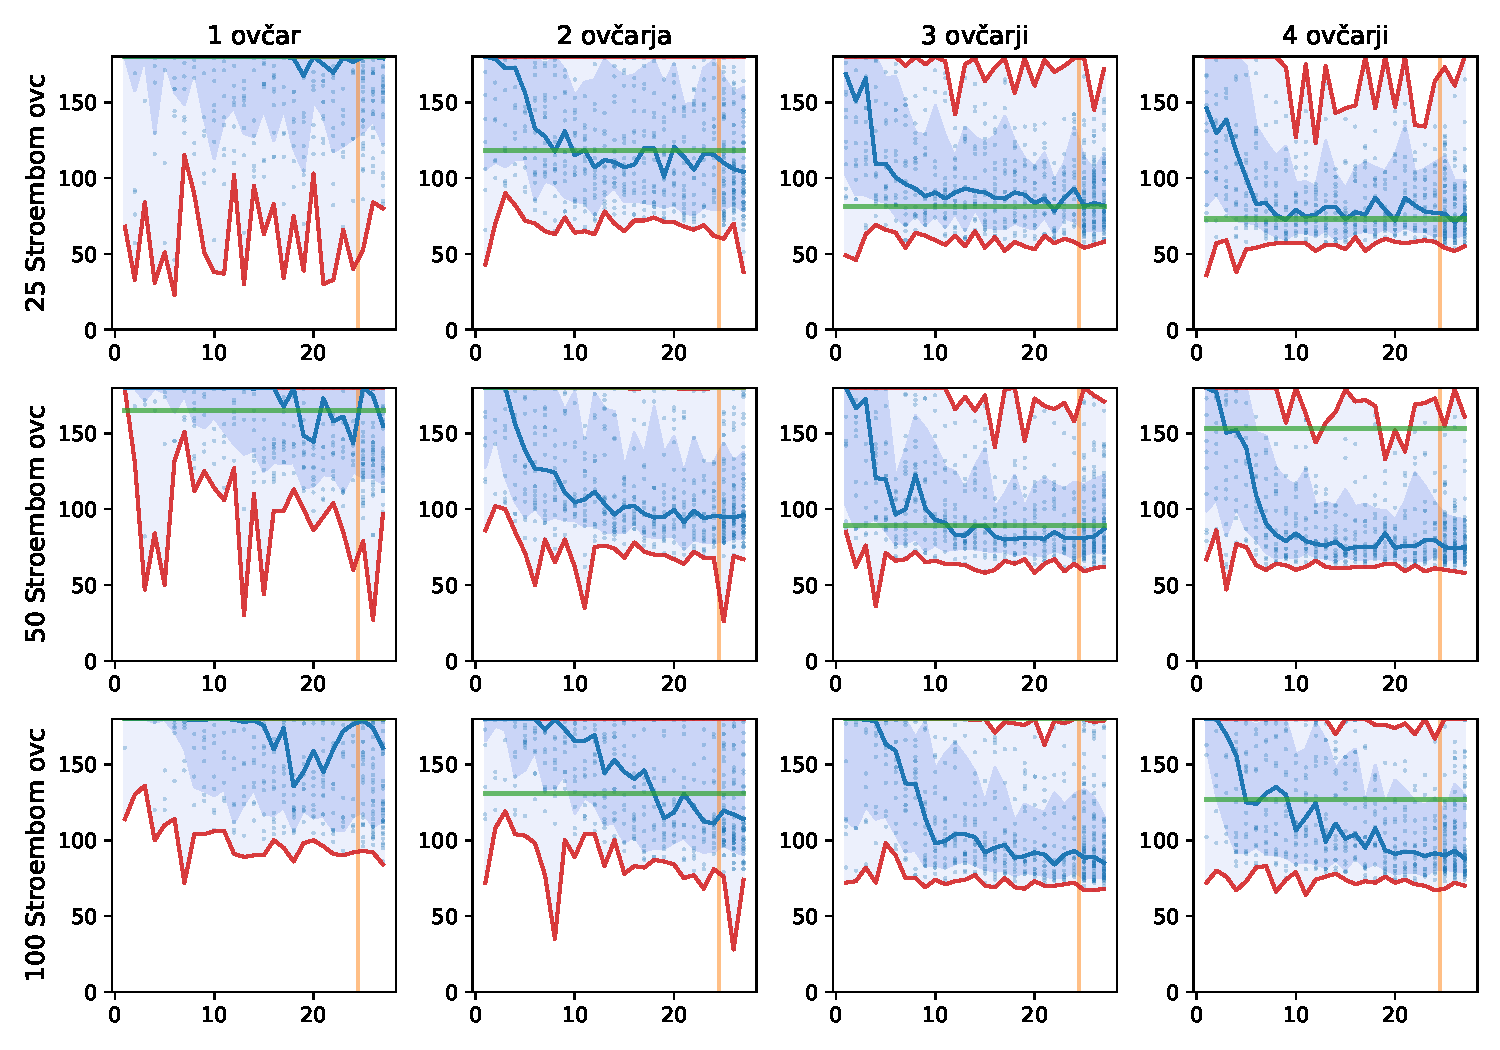
\includegraphics[height=0.4\textheight]{../poglavja/grafi/Stroembom-evolucija-MaxT.pdf}
\caption[Trajanje simulacije skozi generacije]{Trajanje simulacije skozi generacije. Rezultati so pričakovani glede na ocenjeno uspešnost na sliki~\ref{fig:fit}. Na večini grafov opazimo, da je mediana na koncu blizu minimalnega časa. Trajanje simulacije je navzdol omejeno s hitrostjo črede. Hitrost teka je pri ovcah po obeh modelih enaka, ampak je čreda ovc po Str{\"o}mbomovem modelu počasnejša zaradi tresenja, katerega smo se želeli znebiti z uvedbo popravljenega modela.} % narejena je s programom Inkscape
\label{fig:maxt}
\end{figure}

\begin{figure}[H]  % ali t za na vrhu ali h! za točno tukaj
	\centering
	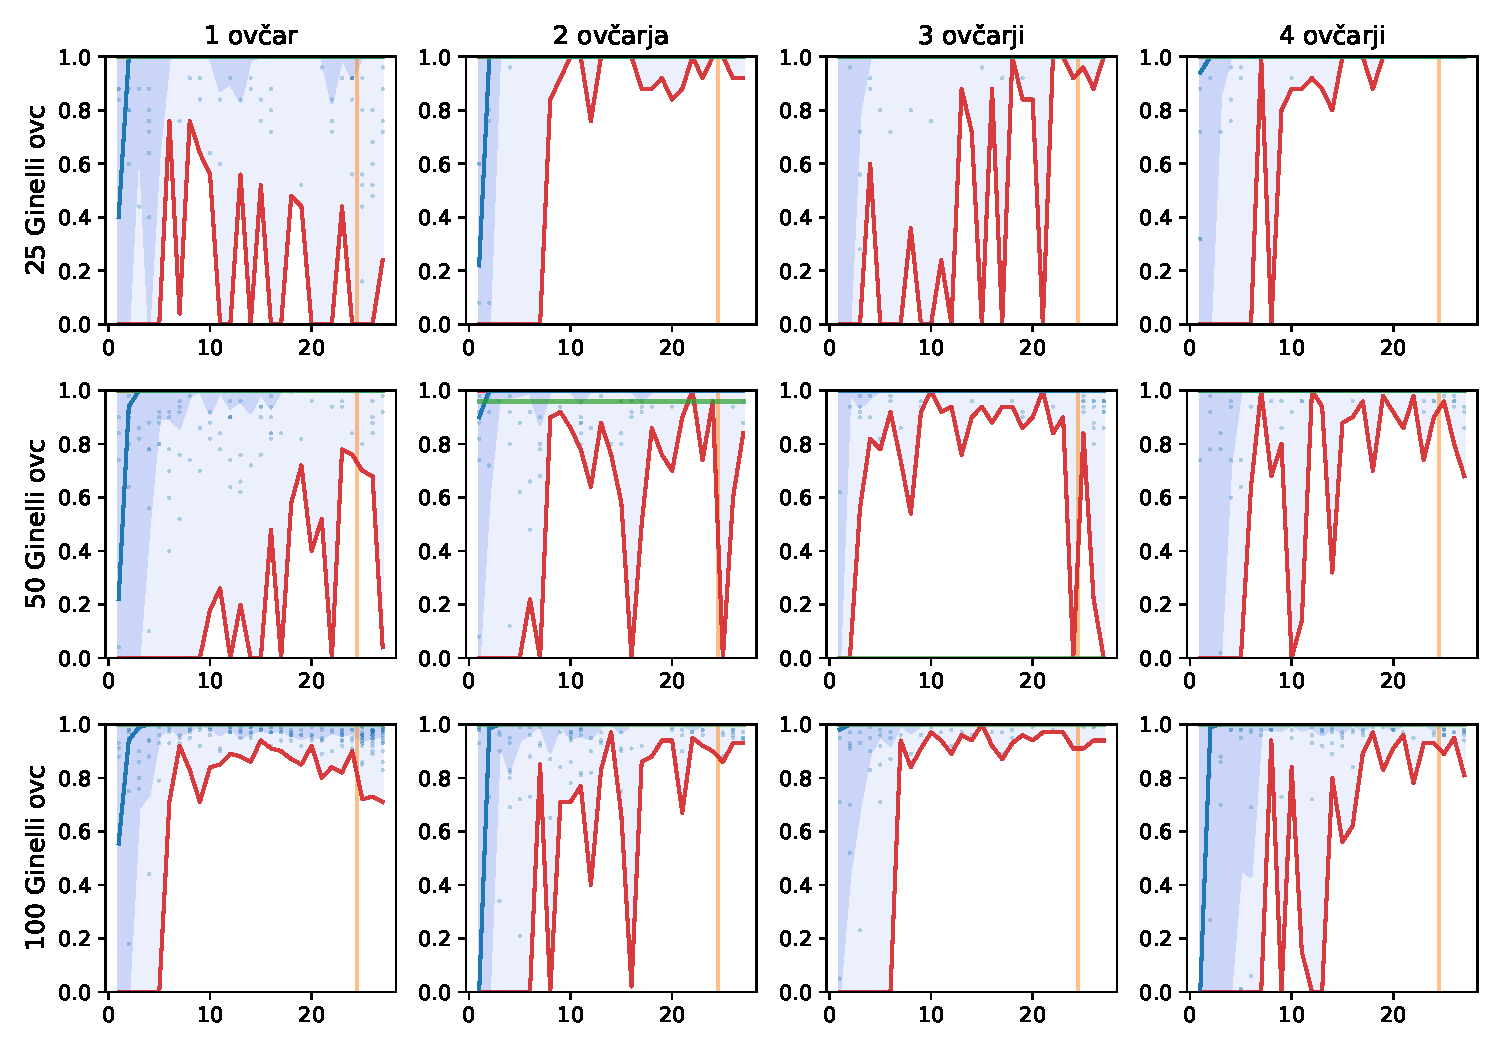
\includegraphics[height=0.4\textheight]{../poglavja/grafi/Ginelli-evolucija-Uspeh.pdf}
	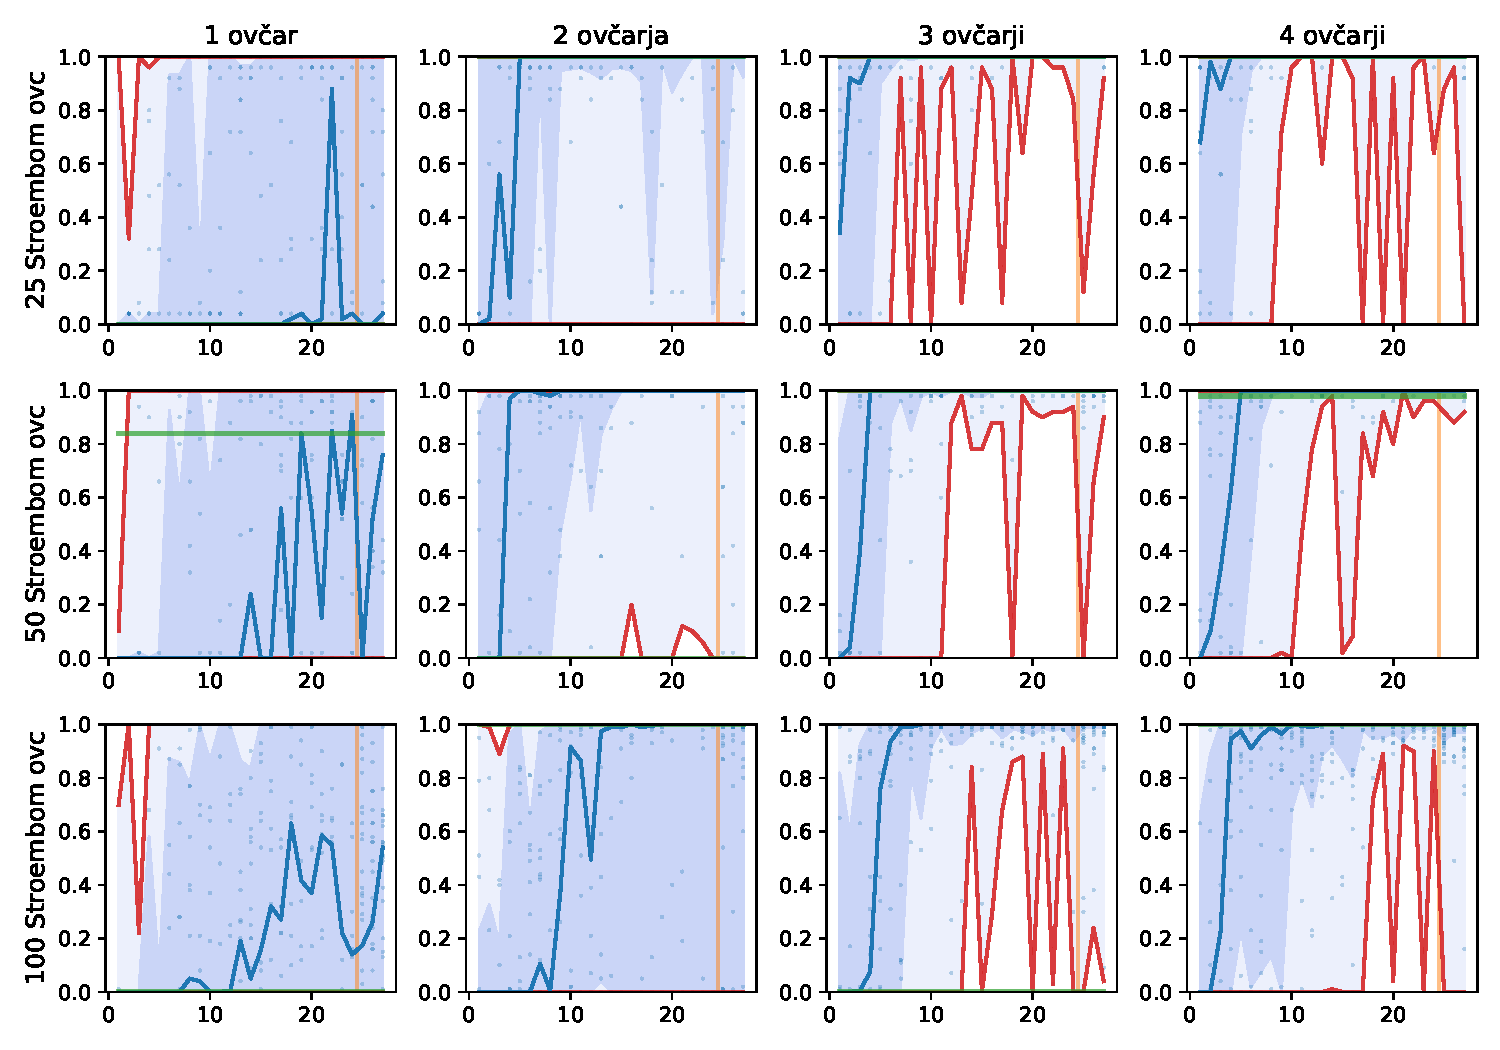
\includegraphics[height=0.4\textheight]{../poglavja/grafi/Stroembom-evolucija-Uspeh.pdf}
	\caption[Delež ovc v staji ob koncu skozi generacije]{Delež ovc v staji ob koncu skozi generacije. Opazimo, da v večini primerov mediana pride vsaj blizu 100~\%, za čredo ovc po Ginellijevem modelu pa se tej vrednosti približa tudi minimum, kar pomeni, da le redko ovčarjem ne uspe privesti vseh ovc v stajo, ampak tudi tedaj jih je na pašniku le še nekaj. Višje število ovčarjev pozitivno vpliva na delež ovc v staji ob koncu simulacije.} % narejena je s programom Inkscape
	\label{fig:uspeh}
\end{figure}

\begin{figure}[H]  % ali t za na vrhu ali h! za točno tukaj
\centering
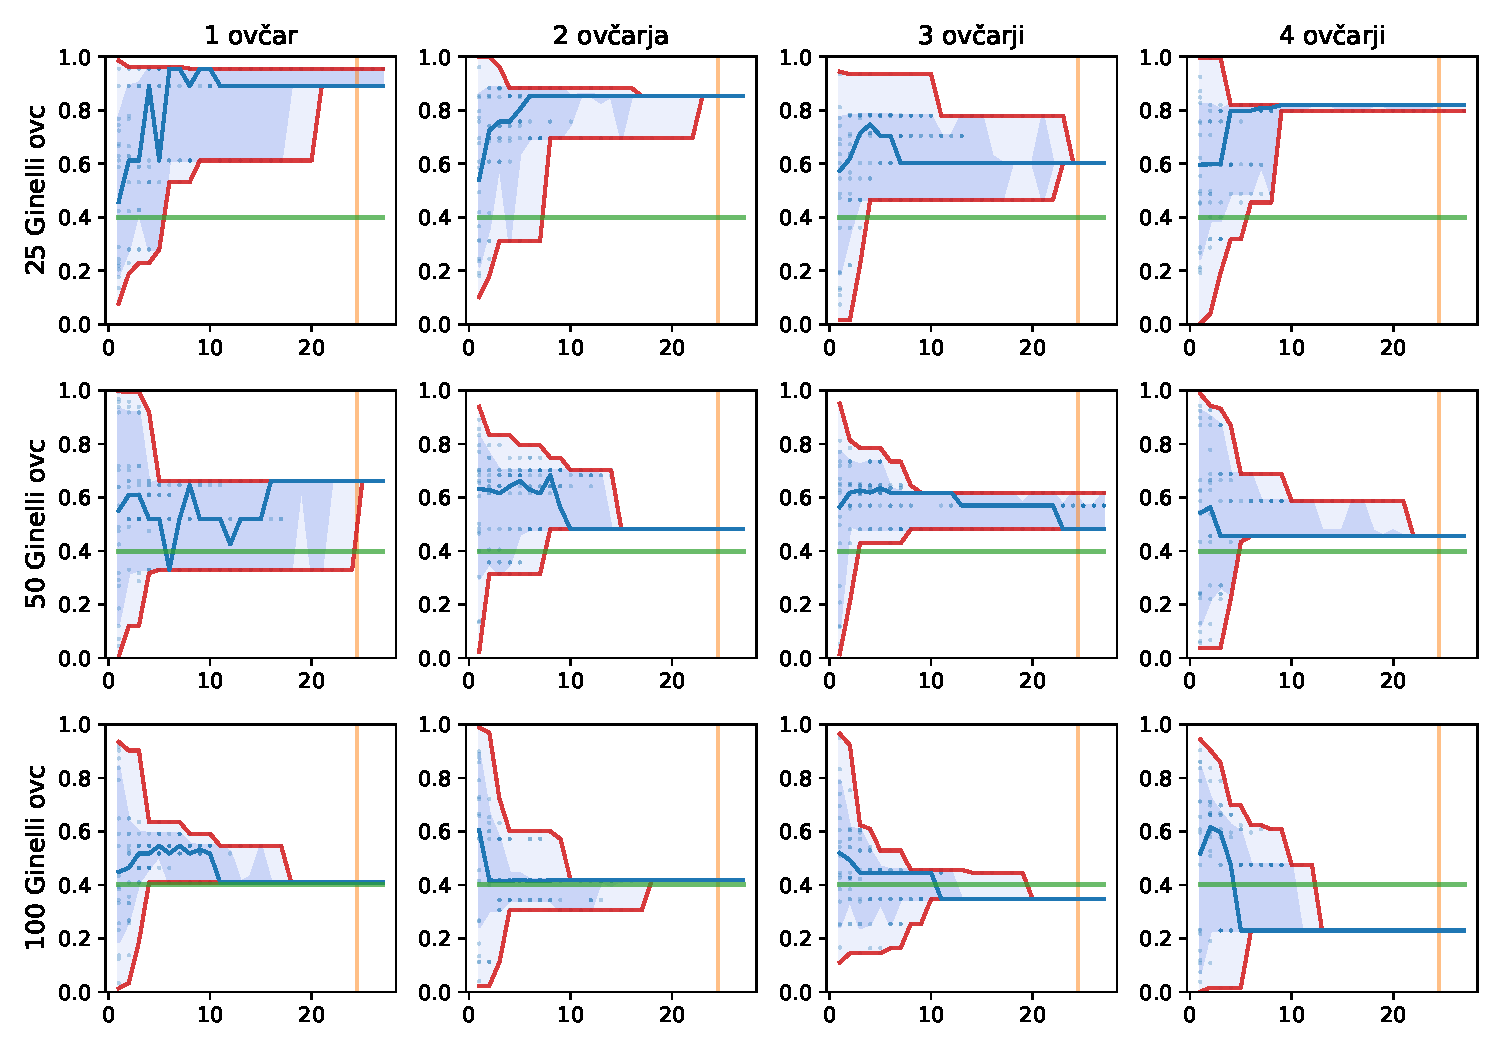
\includegraphics[height=0.4\textheight]{../poglavja/grafi/Ginelli-evolucija-Gen2.pdf}
\caption[Vrednost genotipa za parameter $r_a$ skozi generacije]{Vrednost genotipa za parameter $r_a$ skozi generacije. Sčasoma večina genotipov izumre in ostane le še majhna variabilnost, ki bi se tudi sčasoma zmanjšala. Neželenim izumrtjem bi se do neke mere lahko izognili z mutacijami na celotnem intervalu, kot je to običajno. Naša ideja ožjega intervala je morda naredila nekaj škode pri uspešnosti modela.} % narejena je s programom Inkscape
\label{fig:Ge-gen2}
\end{figure}

\subsection{Model razvit z genetskim algoritmom}

Na sliki~\ref{fig:gen1-4} si lahko ogledamo vrednosti prvih štirih parametrov modela naučene z genetskim algoritmom v odvisnosti od števila ovc in ovčarjev. Pri ostalih parametrih ni videti tako lepe povezave med velikostjo črede in vrednostjo parametra. Na sliki~\ref{fig:lokacije} pa si oglejmo poti agentov med simulacijo.

\begin{figure}[H]  % ali t za na vrhu ali h! za točno tukaj
	\centering
	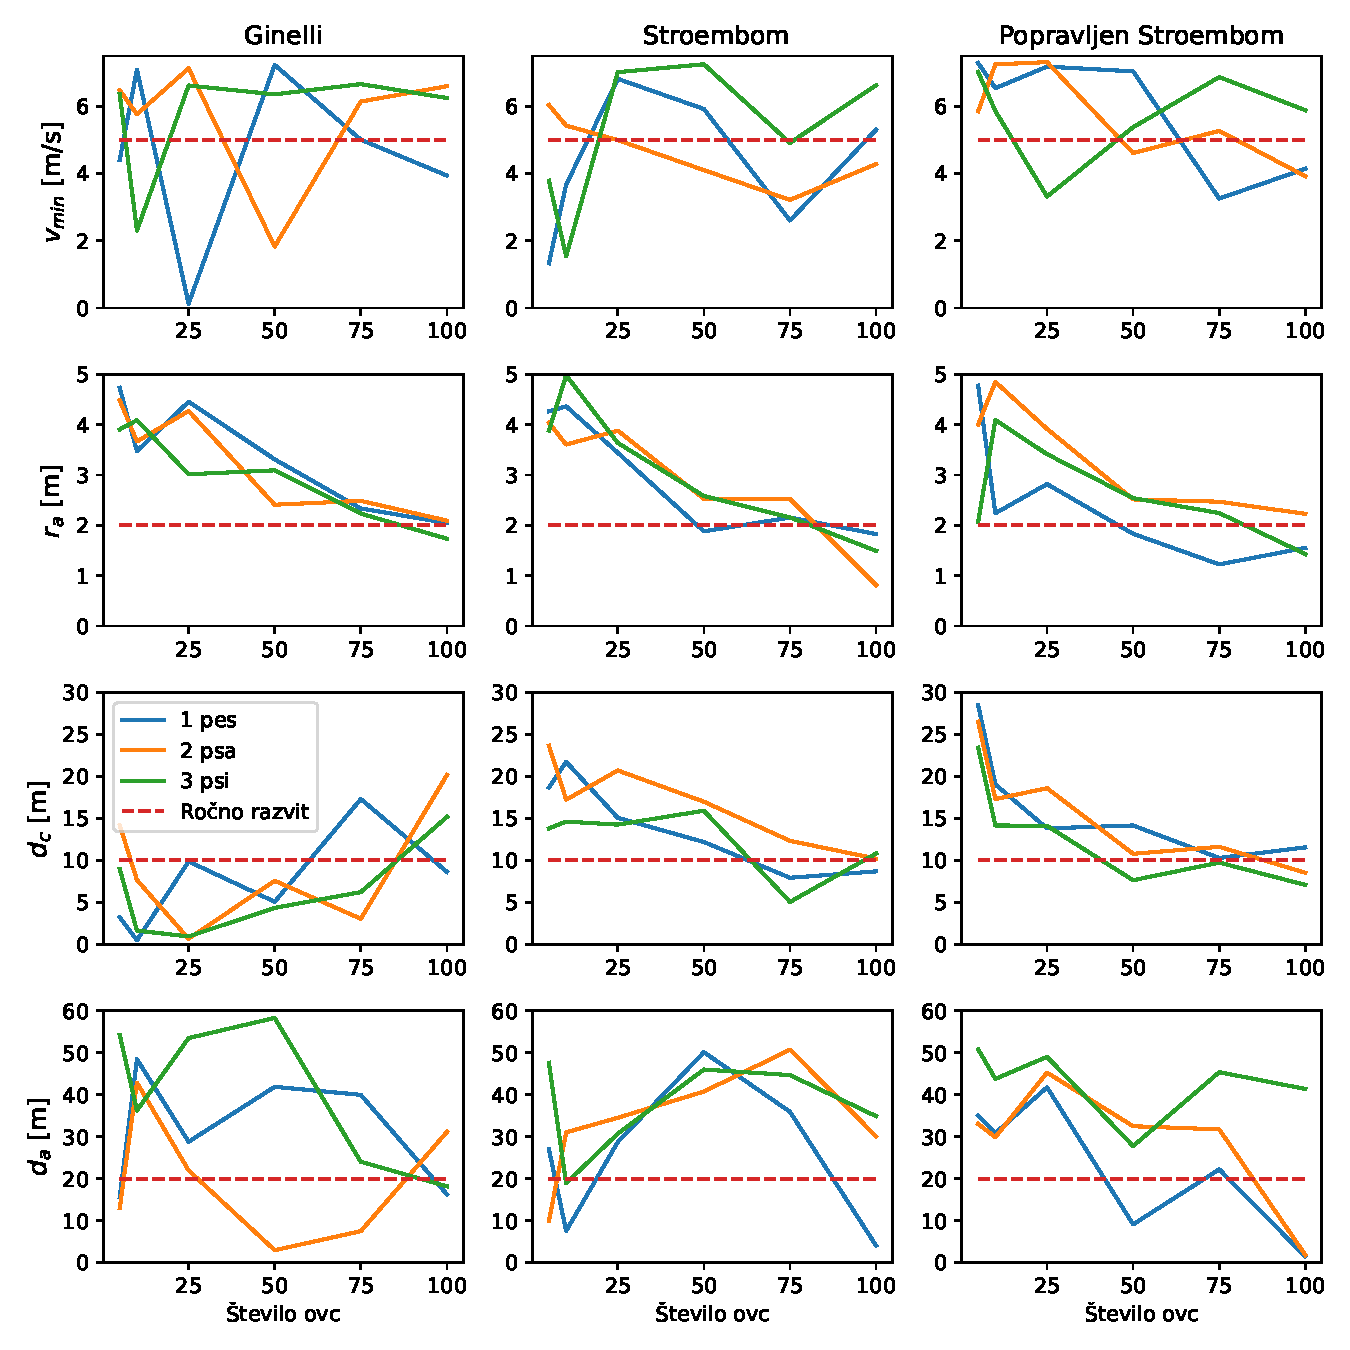
\includegraphics[width=\textwidth]{../poglavja/grafi/geni-1-4.pdf}
	\caption[Naučene vrednosti prvih parametrov]{Naučene vrednosti prvih parametrov. Izbrani parametri predstavljajo hitrost v stanju vodenja, faktor za dovoljeno velikost črede, razdaljo za zbiranje in razdaljo za zaznavo ovc na poti. Vrednosti so si ne glede na število ovčarjev precej podobne. Za večjo čredo pa lahko opazimo, da je vrednost parametra podobna ročno razvitemu modelu. Pri tem modelu smo vrednosti vzeli enake kot avtorji modela. To velja za vse tri modele gibanja ovc. Legenda se nahaja le pri enem grafu, a velja za vse.} % narejena je s programom Inkscape
	\label{fig:gen1-4}
\end{figure}

\begin{figure}[H]  % ali t za na vrhu ali h! za točno tukaj
	\centering
	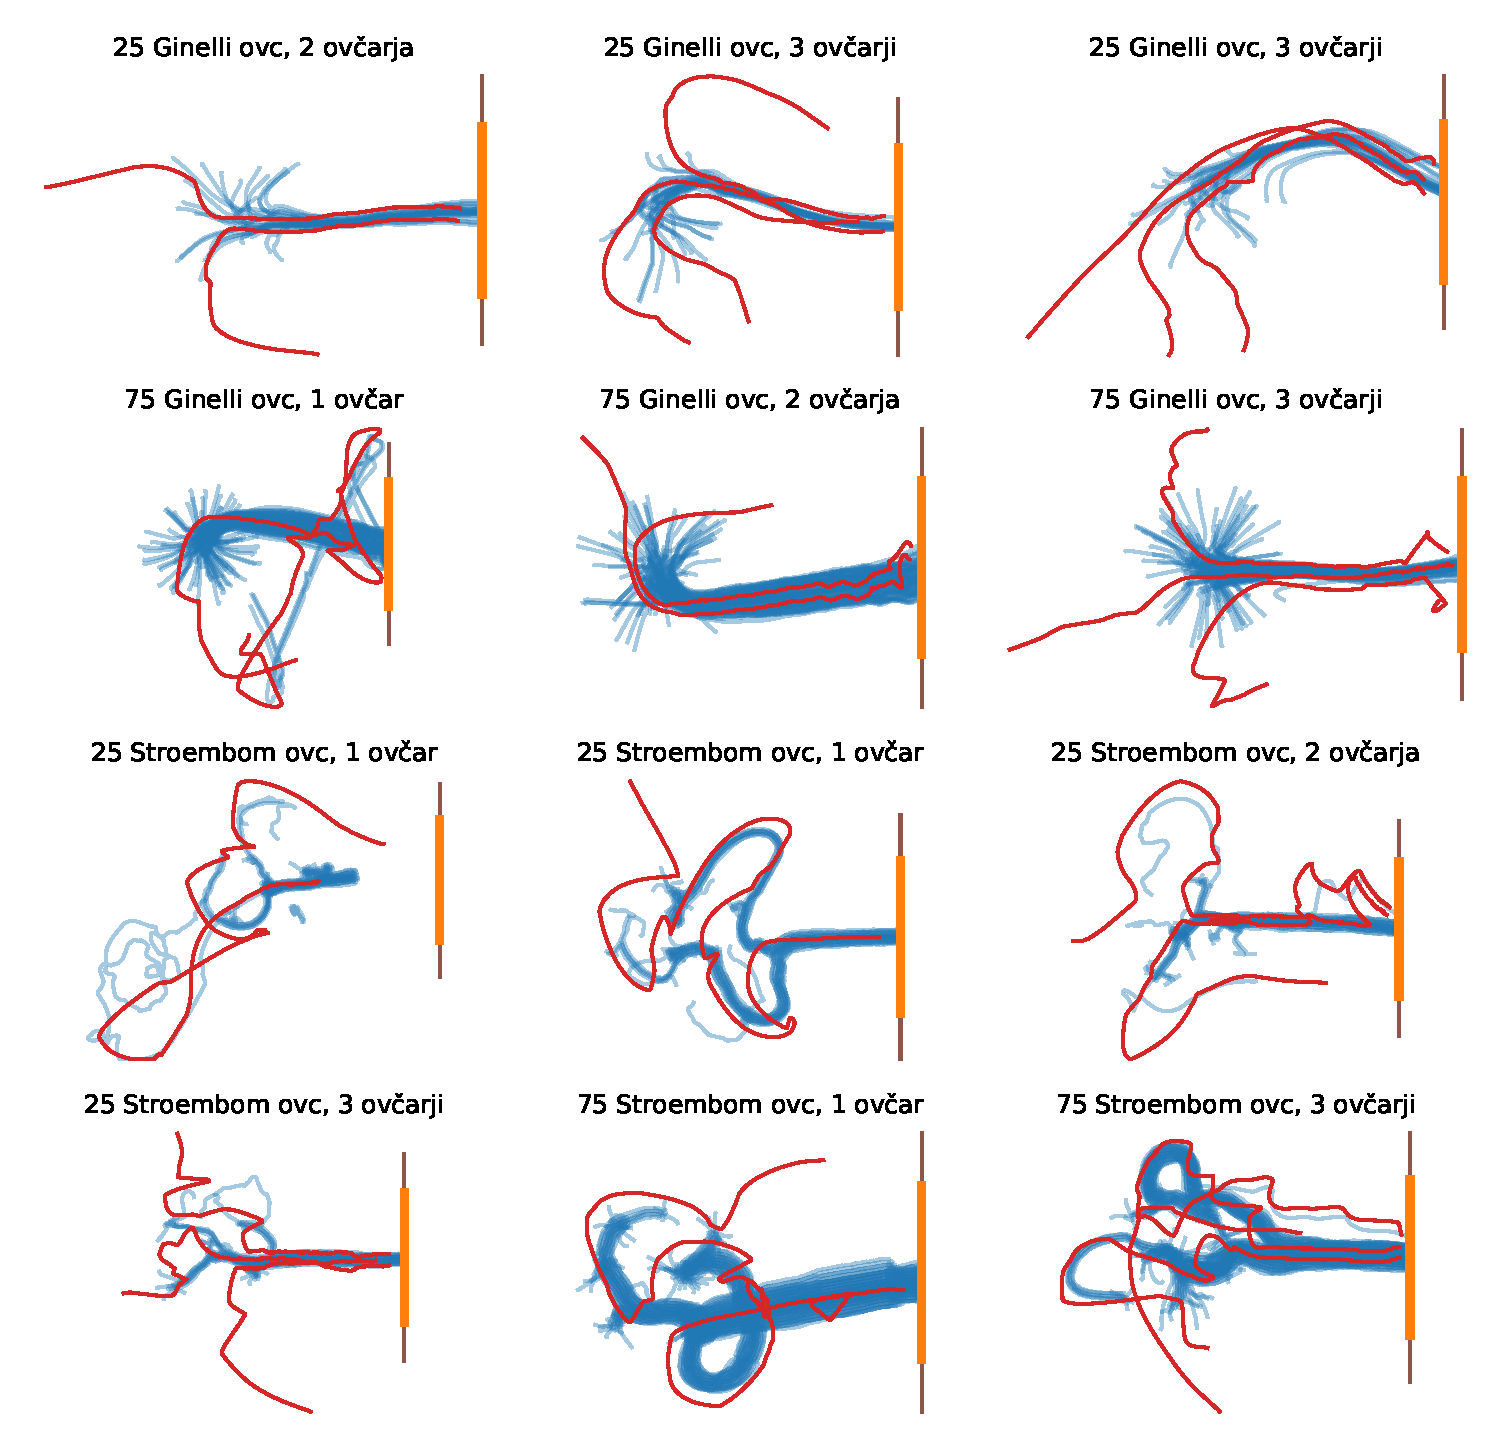
\includegraphics[width=\textwidth]{../poglavja/grafi/lokacijeAI1.pdf}
	\caption[Poti agentov med simulacijo]{Poti agentov med simulacijo. Rdeča krivulja predstavlja pot ovčarja, modra je pot ovce, oranžen pa je vhod v stajo. Opazimo, da se ovce same zberejo že ob približanju ovčarjev, ti pa jim morajo pogosto le še privesti v stajo. Poleg tega se pri ovcah po Ginellijevem modelu le redko zgodi, da bi katera ovca pobegnila stran od črede.} % narejena je s programom Inkscape
	\label{fig:lokacije}
\end{figure}

\subsection{Model z adaptivnim genom}

Nato smo se lotili učenja modela z adaptivnim genom. Zaradi težavnosti učenja se nam je uspelo učiti le na čredi veliki do deset ovc po Ginellijevem modelu. Poleg tega smo se v tem primeru osredotočili na enega samega ovčarja, saj ima ta v preostalih dveh modelih največ težav. Na sliki~\ref{fig:donosnost-nagrade} si lahko ogledamo potek učenja obeh nevronskih mrež.

\begin{figure}[H]  % ali t za na vrhu ali h! za točno tukaj
	\centering
	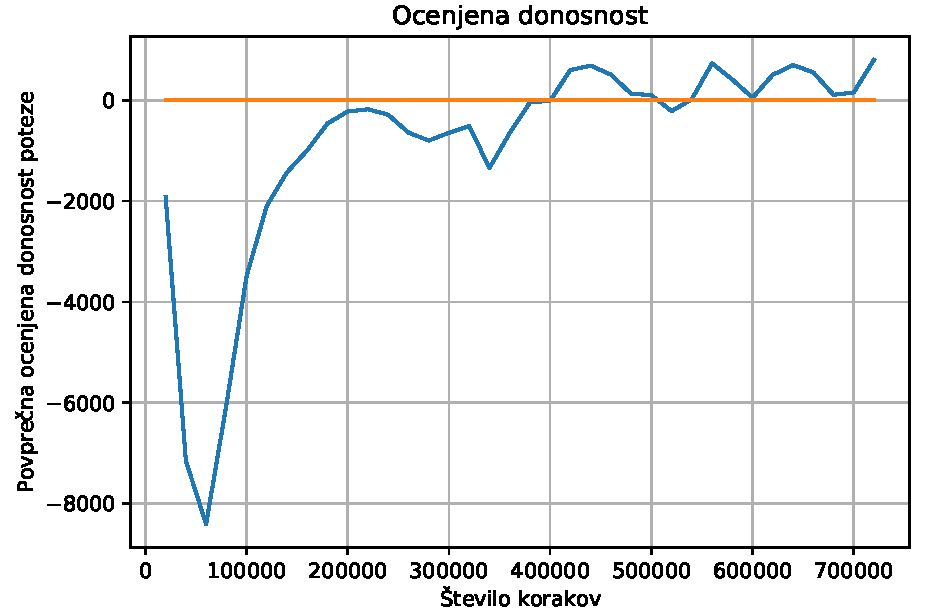
\includegraphics[width=0.49\textwidth]{../poglavja/grafi/donosnostAI2.pdf} 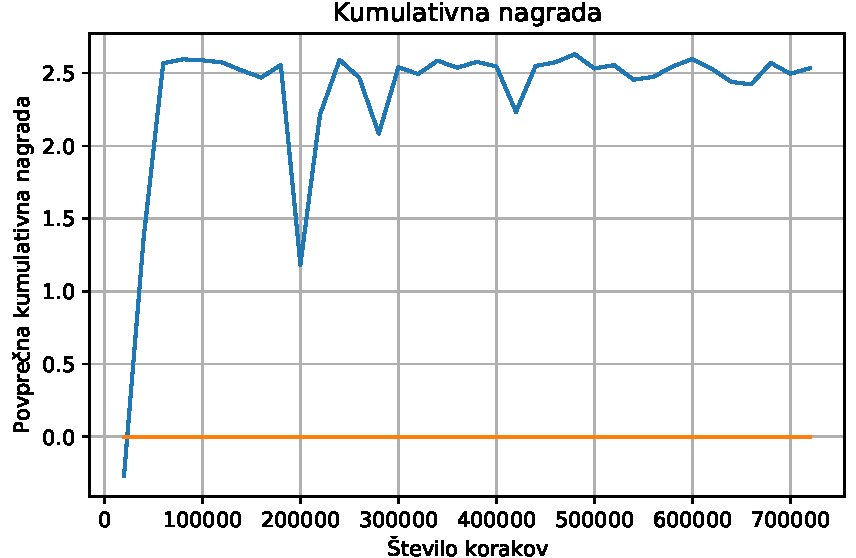
\includegraphics[width=0.49\textwidth]{../poglavja/grafi/nagradeAI2.pdf}
	\caption[Ocenjevanje dobljene nagrade in dejanska dobljena nagrada]{Ocenjevanje dobljene nagrade in dejanska dobljena nagrada. Levi graf nam prikazuje povprečno ocenjeno donosnost poteze, pri čemer model najprej nagrade močno podcenjuje, kasneje pa se jih nauči dobro predvideti. Na desnem grafu pa lahko vidimo hiter vzpon povprečne kumulativne nagrade skozi simulacije in nato le še nekaj padcev uspešnosti zaradi raziskovanja. Ker postaja s časom prostor stanj vedno bolje raziskan, so ti padci kasneje redkejši in manjši.} % narejena je s programom Inkscape
	\label{fig:donosnost-nagrade}
\end{figure}

\subsection{Primerjava modelov vodenja}

Na zadnjih slikah si oglejmo še primerjavo vseh modelov ovc in ovčarjev. Na slikah~\ref{fig:180s} in~\ref{fig:cas} hitro opazimo višjo povprečno uspešnost modela razvitega z genetskim algoritmom v vseh izbranih lastnostih, ampak to le za območje, na katerem smo iskali najboljši gen. Za eno ovco ali ovc več kot 100 pa so rezultati veliko slabši kot pri ročno razvitem modelu, kjer smo vedno vzeli gen za najbolj podobno kombinacijo števila ovc in ovčarjev. To kaže na veliko preprileganje na učni množici, predvsem pri čredah ovc po navadnem in popravljenem Str{\"o}mbomovem modelu. To preprileganje je opazno predvsem pri večjem številu ovčarjev.

Na sliki~\ref{fig:1gin} se osredotočimo le na enega ovčarja in čredo ovc po Ginellijevem modelu, za lažjo primerjavo modelov. Prva dva modela vodenja ovčarja sta namreč za več ovčarjev že dovolj dobra, zato se zdi najbolj smiselno najti model, ki bo uspešen tudi v primeru enega samega ovčarja. Vidimo, da je tudi model z adaptivnim genom popolnoma primerljiv najboljšemu izmed ostalih dveh, razen pri čredi z 200 ovcami. To nam kaže na velik potencial tega modela, saj je dobro posplošil znanje pridobljeno na zelo majhni čredi.

\begin{figure}[ht]  % ali t za na vrhu ali h! za točno tukaj
	\centering
	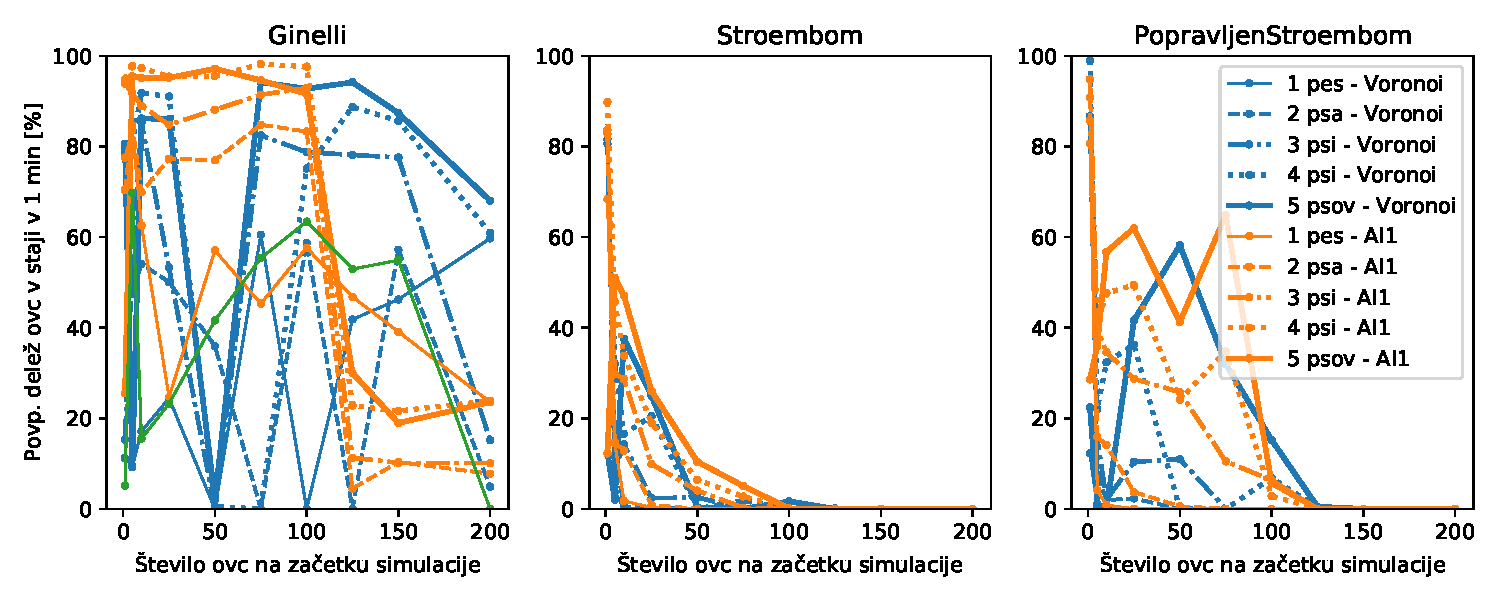
\includegraphics[width=\textwidth]{../poglavja/grafi/povp60s.pdf}
	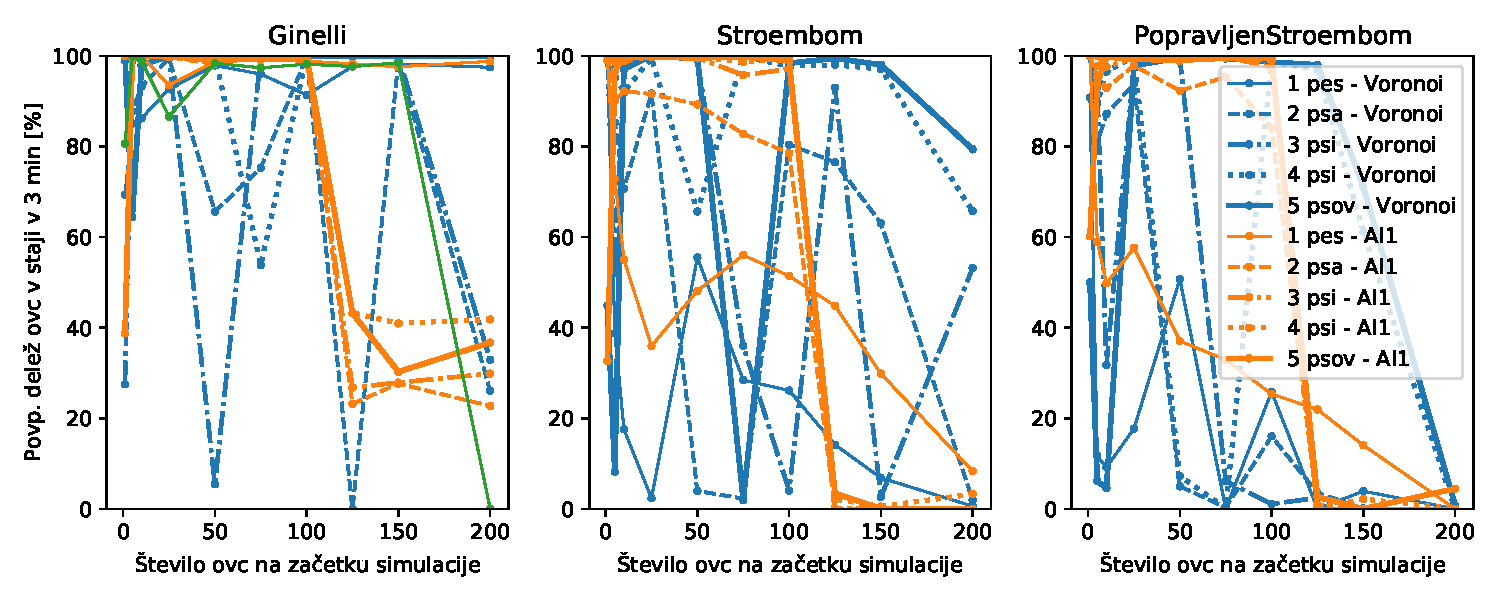
\includegraphics[width=\textwidth]{../poglavja/grafi/povp180s.pdf}
	\caption[Delež ovc v staji za različne črede in število ovčarjev]{Delež ovc v staji za različne črede in število ovčarjev. V zgornji vrsti grafov vidimo povprečen delež ovc v staji po eni minuti simulacije, v spodnji vrsti pa po treh minutah. Ker je čreda počasnejša pri ovcah po Str{\"o}mbomovem modelu, je po eni minuti delež opazno nižji, še posebno za velike črede. Popravljeni model je očitno nekoliko hitrejši, a še vedno zelo podoben.} % narejena je s programom Inkscape
	\label{fig:180s}
\end{figure}

\begin{figure}[ht]  % ali t za na vrhu ali h! za točno tukaj
	\centering
	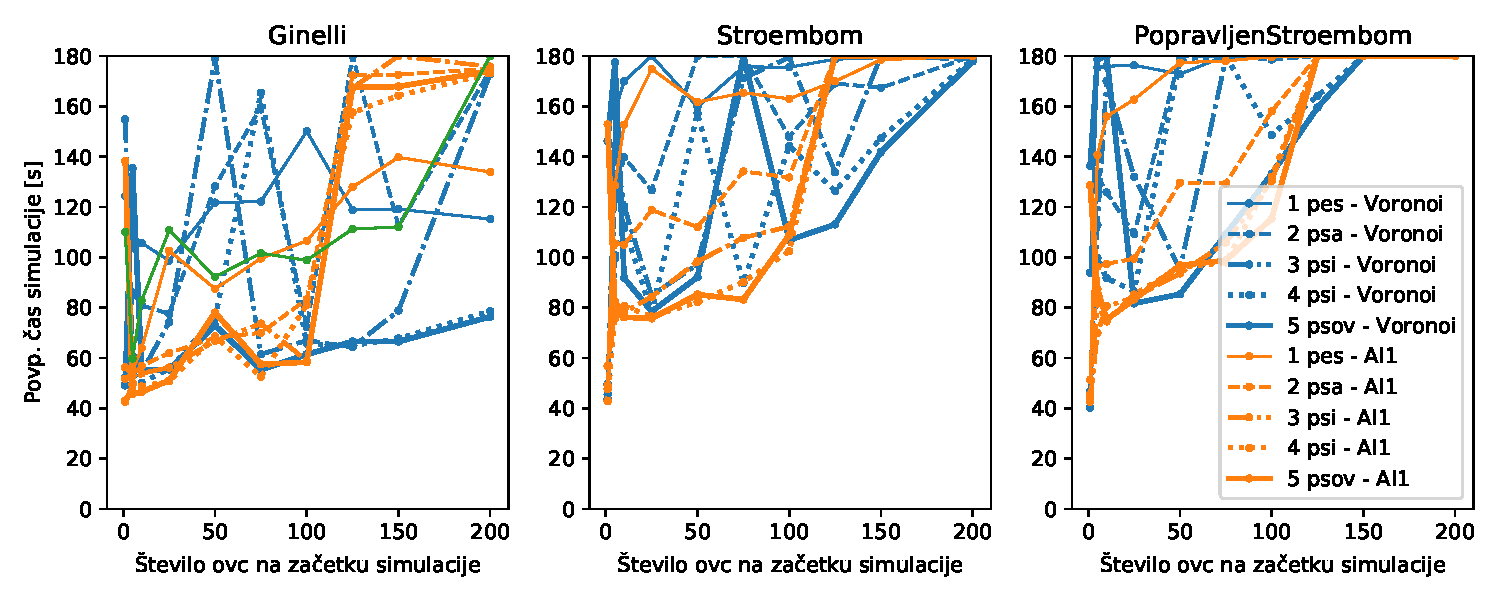
\includegraphics[width=\textwidth]{../poglavja/grafi/cas.pdf}
	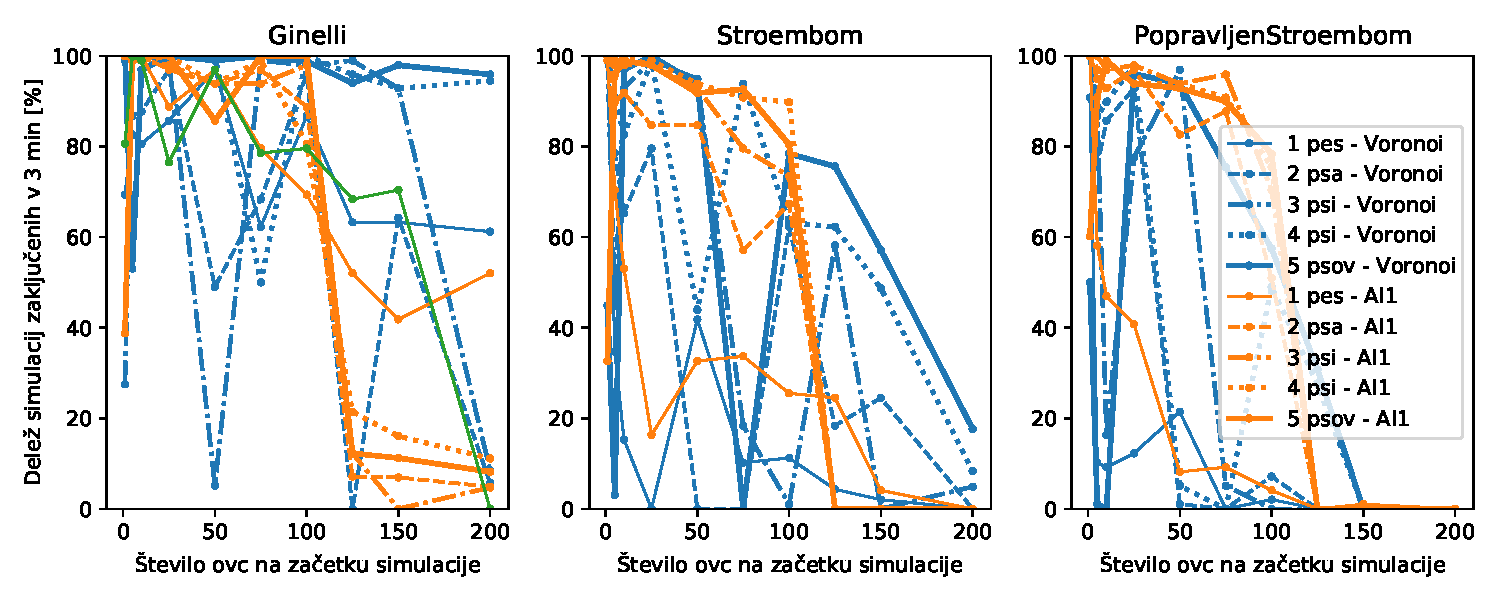
\includegraphics[width=\textwidth]{../poglavja/grafi/zakljucene.pdf}
	\caption[Povprečen čas in delež zaključenih simulacij]{Povprečen čas in delež zaključenih simulacij.} % narejena je s programom Inkscape
	\label{fig:cas}
\end{figure}

\begin{figure}[ht]  % ali t za na vrhu ali h! za točno tukaj
	\centering
	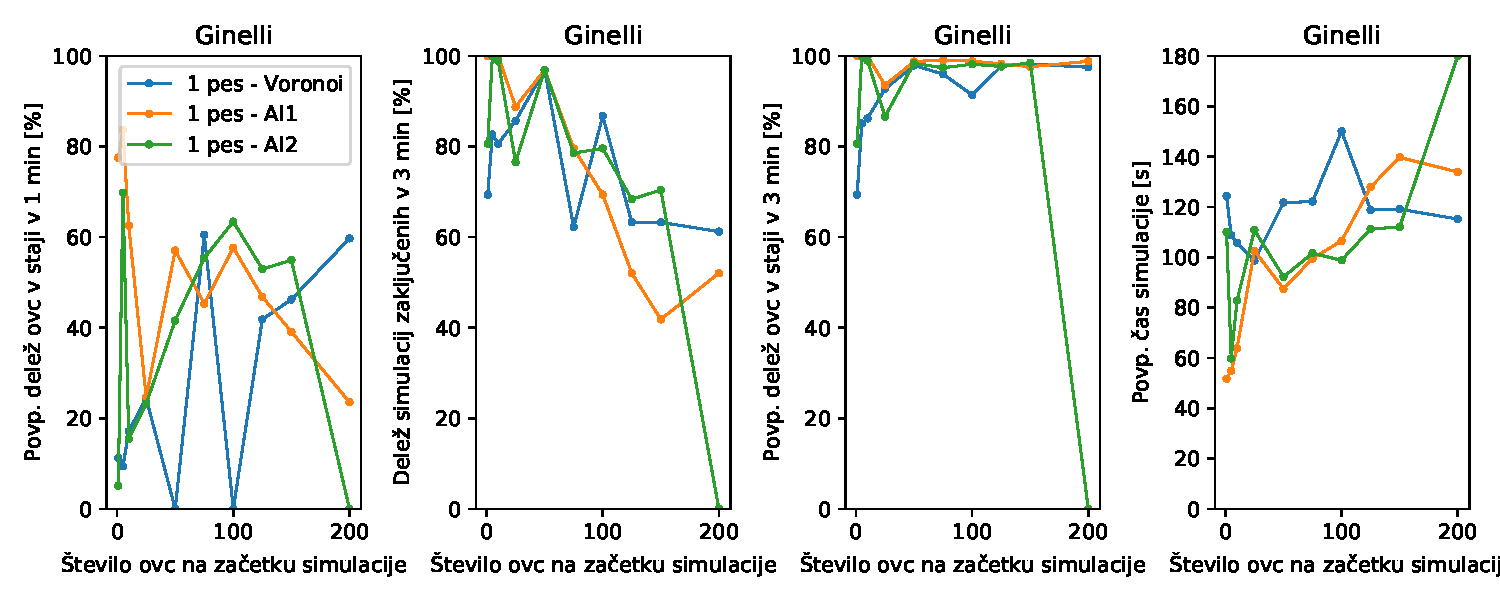
\includegraphics[width=\textwidth]{../poglavja/grafi/1-Ginelli.pdf}
	\caption[Primerjava modelov vodenja enega ovčarja]{Primerjava modelov vodenja enega ovčarja za čredo po Ginellijevem modelu. Opazimo, da je model z adaptivnim genom primerljiv ali celo boljši kot najboljši izmed ostalih dveh modelov. Njegova uspešnost presega ostala dva še posebej pri čredi 100-150 ovc. Za manjše črede pa je običajno najuspešnejši model razvit z genetskim algoritmom.} % narejena je s programom Inkscape
	\label{fig:1gin}
\end{figure}

\subsection{Razprava}

Kot pričakovano je vsak naslednji model v nečem boljši, je pa problem modela razvitega z genetskim algoritmom, da se ne prilagaja spreminjanju velikosti črede, ter ne opazuje oddaljenosti od ovc. Zelo pa je pomembno kako daleč je ovčar od črede, da jo še lahko vodi. V tem smislu, se je za odličnega izkazal model z adaptivnim genom, ki je vse to upošteval. Težava tega modela pa je zamudno in nestabilno učenje, zaradi katerega je težko pridobiti dober model naučen na večjih čredah. Za to bi potrebovali veliko časa in pametno nastavljene parametre PPO algoritma.

Ideja sodelovanja ovčarjev se je izkazala za dobro vsaj pri ovcah po Ginellijevem modelu. Za ostala dva modela pa bi bilo bolje, če bi si ovčar izbral del črede, ki se drži skupaj in ga pripeljal bliže drugemu delu dokler ne bi zbral vseh ovc v eno čredo. Zdaj se namreč pogosto zgodi, da pride v ravnovesno stanje in stoji med čredama ali se brez koristi sprehaja od ene do druge. To bi lahko rešili z računanjem gruč in določanjem, katero gručo vodi kateri ovčar, dokler ni celotna čreda v eni sami gruči.

